\section{Misura di Lebesgue}
\chapquote{``No one shall expel us from the paradise which Cantor has created for us."}{David Hilbert}

\subsection{Verso la misura di Lebesgue}
Vorremmo definire una misura $\lambda$ su $\mathbb R$ o $\mathbb R^n$ tale che, per ogni $a<b$,
\begin{enumerate}
    \item Misuri la lunghezza di un qualsiasi intervallo \\ $\lambda((a,b))=b-a$
    \item Sia invariante rispetto alla traslazione \\$\forall E, \lambda(E+x)=\lambda(E)$
\end{enumerate}
\subsubsection{(thm) Teorema di Ulam}
L'unica misura definita sul power set di $\mathbb R$ che soddisfa la condizione $\lambda(\{a\})=0\quad \forall a\in \mathbb R$ è la misura banale.
\subsubsection{(def) Outer measure}
Una misura esterna su $X$ è una funzione $$\mu^*:\mathcal P(X)\to [0,+\infty]$$ tale che:
\begin{enumerate}
    \item $\mu^*(\emptyset)=0$
    \item è monotona \\ $E\subset F\subset X \implies \mu^*(E)\le \mu^*(F)$
    \item è $\sigma$-subadditiva \\ Data $\{E_n\}_{n\in \mathbb N}\subset \mathcal P(X)$, allora $\mu^*\Big(\bigcup_{n=1}^{+\infty} E_n\Big)\le \sum_{n=1}^{+\infty}\mu^*(E_n)$
    
\end{enumerate}
Osserviamo che qualsiasi misura $\mu$ sul power set di $X$ è anche una outer measure su $X$.

\subsubsection{(prop) Costruzione di una outer measure}\label{(prop) Costruzione di una outer measure}
Per costruire una outer measure è possibile partire da una funzione su alcuni set "elementari".
Sia $\mathcal E \subset \mathcal P(X)$ e sia $f:\mathcal E \to [0,+\infty]$ una funzione.
\\
Assumendo che la famiglia $\mathcal E$ contenga l'insieme vuoto e l'insieme $X$. Assumendo inoltre che $f(\emptyset)=0$,\\
Allora, $\forall E\subset X$, possiamo definire
$$\mu^*(E)=\inf\Big\{\sum_{n=1}^{+\infty}f(A_n), \text{ dove } A_n\in \mathcal E \text{ e }E\subset \bigcup_n A_n\quad \forall n\Big \}$$
Allora $\mu^*(E)$ è una outer measure su $X$.
\subsubsection{(def) Caratheodory's condition}
Sia $\mu^*$ una outer measure sul power set $\mathcal P(X)$.
Un set $E\subset X$ si dice $\mu^*$-misurabile se $\forall A\subset X$ si ha:
$$\mu^*(A)=\mu^*(A\cap E)+\mu^*(A\cap E^C)$$
\subsubsection{(lemma) Caratheodory's equivalent condition (*)}
$E$ è $\mu^*$-misurabile
$$\iff$$
$$\forall A \subset X,\ \mu^*(A)<+\infty \implies \mu^*(A)\ge \mu^*(A\cap E)+\mu^*(A\cap E^C)$$
\subsubsection{(thm) Teorema di Carathéodory (*)}
Preso $\mu^*$ outer measure sul power set di $X$,\\
La famiglia $$\mathcal M =\{E \subset X : E \text{ è } \mu^*\text{-misurabile}\}$$
è una $\sigma$-algebra, e $\mu=\mu^*\vert_{\mathcal M}$ è una misura completa.
\paragraph{Alternative statement}
Let $\mathcal A$ be an algebra of subset of a set $X$, and let $\mu$ be a pre-measure defined on $\mathcal A$.

If $\mu$ is $\sigma$-finite ($X$ can be decomposed into a countable union of subsets with finite measure), then:
\begin{enumerate}
    \item There exists an extension of $\mu$ to a measure on the smallest $\sigma$-algebra containing $\mathcal A$, that is the $\sigma$-algebra generated by $\mathcal A$: $\sigma(\mathcal A)$.
    \item This extension is unique.
\end{enumerate}
Carathéodory's theorem guarantees that any pre-measure defined on a smaller collection of sets can be extended to a complete measure on the $\sigma$-algebra generated by those sets.
\subsection{Lebesgue's Measure}
\subsubsection{(def) Misura di Lebesgue su $\mathbb R$}\label{(def) Misura di Lebesgues R}
\begin{enumerate}
    \item Scegliamo $X=\mathbb{R}$, $\mathcal E=\{$intervalli aperti di $\mathbb R\}$ e una funzione f tale che esprima la lunghezza di un intervallo (eg. intervallo aperto $(a,b)$ con $a<b$, $f((a,b))=b-a$).
    \item costruiamo la Lebesgue's outer measure $\lambda^*$ seguendo la proposizione \ref{(prop) Costruzione di una outer measure} 
    \item applichiamo ora il Teorema di Caratheodory sfruttando la outer measure appena creata e otteniamo lo spazio $(\mathbb R, \mathcal L(\mathbb R),\lambda)$ dove $\mathcal L(\mathbb R)$ è la Lebesgue sigma algebra, mentre $\lambda$ è la misura di Lebesgue.
\end{enumerate}
\subsubsection{(def) Misura di Lebesgue su $\mathbb R^n$}
Il procedimento è analogo a quello mostrato in \ref{(def) Misura di Lebesgues R}, scegliendo però $\mathcal E=\{$ rettangoli aperti di $\mathbb R^2\}$ oppure $\{$palle aperte di $\mathbb R^3\}$, ...
\subsubsection{(prop) misura di Lebesgue su insiemi numerabili (*)}
La misura di Lebesgue applicata a un insieme alpiù numerabile è pari a zero.
Si ha infatti che:
\begin{enumerate}
    \item $a\in \mathbb R \implies \{a\}\in\mathcal L(\mathbb R) \ \text{e} \ \lambda(\{a\})=0$
    \item $E\subset \mathbb R$, alpiù numerabile. $\implies E\in \mathcal L(\mathbb R=)$ e $\lambda(E)=0$
\end{enumerate}
\subsubsection{(prop) Borel's vs Lebesgue's sigma algebras (*)}
$$\mathcal B(\mathbb R)\subset \mathcal L(\mathbb R)$$
\subsubsection{(prop) Regolarità della misura di Lebesgue}
Presi $E\subset \mathbb R$, le seguenti proprietà sono equivalenti:
\begin{enumerate}[label=(\roman*)]
    \item $E\in \mathcal L(\mathbb R)$
    \item $\forall \varepsilon>0$, $\exists A \subset \mathbb R$ aperto tale che:
    \begin{itemize}
        \item $E\subset A$
        \item $\lambda^*(A\setminus E)\le \varepsilon$
    \end{itemize}
    \item $\exists G\subset \mathbb R$ di classe $G_\delta$ tale che:
        \begin{itemize}
            \item $E\subset G$
            \item $\lambda^*(G\setminus E)=0$
        \end{itemize}
    \item $\forall \varepsilon >0$, $\exists C\subset \mathbb R$ chiuso tale che:
    \begin{itemize}
        \item $C\subset E$
        \item $\lambda^*(E\setminus C)\le \varepsilon$
    \end{itemize}
    \item $\exists F\subset \mathbb R$, di classe $F_\delta$ tale che:
    \begin{itemize}
        \item $F\subset E$
        \item $\lambda^*(E\setminus F)=0$
    \end{itemize}
\end{enumerate}
\subsection{Non measurable sets}
\subsubsection{(lemma) Lebesgue-negligible sets}
Sia $E\subseteq \mathbb R$ un insieme misurabile e limitato. Si supponga che esista un insieme infinito numerabile limitato $\Sigma \subseteq \mathbb R$ per il quale $\{\sigma +E\}_{\sigma \in \Sigma}$ è una famiglia di insiemi disgiunti.
Allora, $$\lambda(E)=0$$
\subsubsection{(thm) Vitali theorem}
Qualsiasi insieme Lebesgue misurabile $E\subseteq \mathbb R$ con $\lambda(E)>0$ contiene un sottoinsieme che non è Lebegue misurabile.
\newpage
\subsubsection{(def) Insiemi di Cantor}

L'insieme di Cantor \( C \) è un esempio di insieme frattale che si costruisce iterativamente a partire dall'intervallo chiuso \([0, 1]\).

\paragraph{Costruzione dell'insieme di Cantor}

L'insieme di Cantor può essere costruito come segue:
\begin{itemize}
    \item \textbf{Passo 0:} Si parte con l'intervallo \([0,1]\).
    
    \begin{center}
        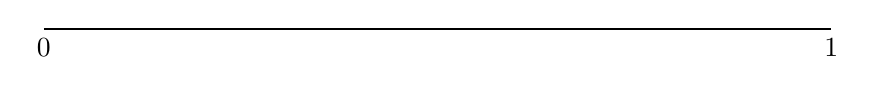
\begin{tikzpicture}
            \draw[thick] (0,0) -- (10,0);
            \node[below] at (0,0) {0};
            \node[below] at (10,0) {1};
        \end{tikzpicture}
    \end{center}

    \item \textbf{Passo 1:} Si rimuove il terzo centrale \(\left( \frac{1}{3}, \frac{2}{3} \right)\).
    
    \begin{center}
        \begin{tikzpicture}
            \draw[thick] (0,0) -- (3,0);
            \draw[thick] (7,0) -- (10,0);
            \node[below] at (0,0) {0};
            \node[below] at (3,0) {$\frac{1}{3}$};
            \node[below] at (7,0) {$\frac{2}{3}$};
            \node[below] at (10,0) {1};
        \end{tikzpicture}
    \end{center}
    
    \item \textbf{Passo 2:} Si rimuovono i terzi centrali da ciascun intervallo rimasto, \(\left( \frac{1}{9}, \frac{2}{9} \right)\) e \(\left( \frac{7}{9}, \frac{8}{9} \right)\).
    
    \begin{center}
        \begin{tikzpicture}
            \draw[thick] (0,0) -- (1,0);
            \draw[thick] (2,0) -- (3,0);
            \draw[thick] (7,0) -- (8,0);
            \draw[thick] (9,0) -- (10,0);
            
            \node[below] at (0,0) {0};
            \node[below] at (1,0) {$\frac{1}{9}$};
            \node[below] at (2,0) {$\frac{2}{9}$};
            \node[below] at (3,0) {$\frac{1}{3}$};
            \node[below] at (7,0) {$\frac{2}{3}$};
            \node[below] at (8,0) {$\frac{7}{9}$};
            \node[below] at (9,0) {$\frac{8}{9}$};
            \node[below] at (10,0) {1};
        \end{tikzpicture}
    \end{center}
    
    \item \textbf{Passi successivi:} Il processo continua indefinitamente, rimuovendo il terzo centrale da ciascun intervallo rimanente.
\end{itemize}
L'insieme che rimane alla fine di questo processo è l'insieme di Cantor.\\
Formalmente, possiamo vedere l'insieme di Canor come l'intersezione numerabile degli insiemi $C^{(i)}$ ottenuti ad ogni passo:
$$C=\bigcap_{n\in \mathbb N} C^{(n)}$$


\begin{figure}[H] % [H] makes sure the figure is placed exactly here
    \centering
    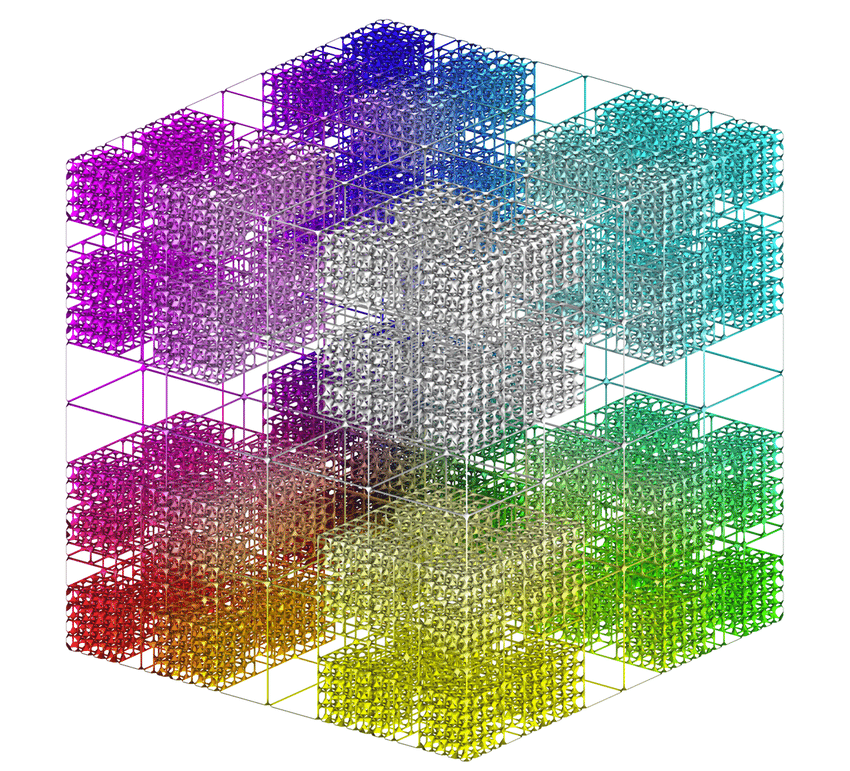
\includegraphics[width=0.4\textwidth]{assets/Three-dimensional-Cantor-set-FMM-tree-for-N-4096-t-1-and-d-H-2-For.png}
    \caption{Polvere di Cantor (Pouransari, Hadi and Darve, Eric, 2015) \cite{article}
}
    \label{fig:example_image}
\end{figure}
\subsubsection{(prop) Proprietà degli insiemi di Cantor}
\begin{enumerate}
    \item $C$ ha la cardinalità del continuo
    \item $C$ ha misura di Lebesgue pari a 0.\\$$\lambda(C)=0$$
    \item $C$ è compatto
    \item $C$ non ha punti interni
    \item $\exists E\subset C$ tale che $E\in \mathcal L(\mathbb R)$ ma $E\notin \mathcal B(\mathbb R)$
\end{enumerate}
\subsection{Funzioni misurabili e integrabili}
\subsubsection{(def) Funzione misurabile}
Siano $(X,\mathcal F)$ e $(Y,\mathcal G)$ due spazi misurabili.\\
Una funzione $f:X\to Y$ viene detta misurabile (o anche $(\mathcal {F,G})$-misurabile) se $$f^{-1}(V)\in \mathcal F\quad \forall V\in\mathcal G$$
\subsubsection{(prop) Condizione necessaria e sufficiente per la misurabilità di una funzione (*)}
Siano $(X,\mathcal F)$ e $(Y,\mathcal G)$ due spazi misurabili.\\
Basta verificare che $f$ soddisfi la definizione di misurabilità per ogni elemento di una famiglia di generatori di $\mathcal G$.\\
Sia $\mathcal S\subset \mathcal G$ tale che $\mathcal G=\sigma_0(\mathcal S)$.\\
Allora vale la seguente doppia implicazione:
$$f \text{ è misurabile}\iff f^{-1}(E)\in \mathcal F\quad  \forall E\in \mathcal S$$
\subsubsection{(def) Borel misurabilità}
Una funzione $f:X\to Y$ si dice Borel misurabile se è $(\mathcal B(X),\mathcal B(Y))$-misurabile.
\subsubsection{(def) Lebesgue misurabilità}
Una funzione $f:X\to Y$ si dice Borel misurabile se è $(\mathcal M,\mathcal B(Y))$-misurabile.\\
Dove $\mathcal M$ è un'insieme che contiene $\mathcal B(X)$, ad esempio:
\begin{itemize}
    \item $\mathcal M=\mathcal B(X)$
    \item $\mathcal M=\mathcal P(X)$
    \item $\mathcal M=\mathcal L(X)$
    \item etc...
\end{itemize}
(oss) Notiamo quindi che la Lebesgue misurabilità implica la Borel misurabilità.
\subsubsection{(prop) continuità e misurabilità di una funzione (*)}
Sia $f:X\to Y$ una funzione continua, allora è anche Borel misurabile e, di conseguenza, Lebesgue misurabile. 
\subsubsection{(prop) misurabilità della composizione di funzioni (*)}
Sia $f:X\to Y$ una funzione Lebesgue misurabile.
Sia $g:Y\to Z$ una funzione continua.
Allora
$$g\circ f:X\to Z$$ è Lebesgue misurabile.
\subsubsection{(prop) misurabilità di una funzione continua su funzioni misurabili (*) }
Date due funzioni $u,v:X\to \mathbb R\ (\text{or }\bar{\mathbb R}) $ tali che $u$ e $v$ siano Lebesgue measurabili.\\
Presa una funzione $\Phi:\mathbb R^2\to \mathbb R$ continua,\\
Allora la funzione $h:X\to \mathbb R$,$$\ h(x)=\Phi(u(x),v(x))$$ è Lebesgue misurabile.
\subsubsection{(def) almost everywhere holding property}
Sia $(X,\mathcal M, \mu)$ uno spazio di misura completo (\ref{(def) completezza della misura o dello spazio di misura}). \\
Una proprietà $P(x)$ è vera per $\mu$-almost every $x\in X$ o $\mu$-almost everywhere (a.e.) se
$$\mu(\{x\in X:P(x)\text{ is false}\})=0$$
\subsubsection{(prop) misurabilità di funzioni uguali a.e.}
\begin{enumerate}
    \item $f:X\to \bar{\mathbb R}$ tale che $f=g$ a.e. , con $g$ misurabile $\implies f$ è misurabile 
    \item Data una successione di funzioni misurabili $\{f_n\}_{n\in \mathbb N}$ tale che $f_n\to f$ a.e. $\implies f$ è misurabile
\end{enumerate}
\newpage
